\documentclass[11pt,a4paper]{article}
\usepackage[utf8]{inputenc}
\usepackage[margin=0.8in]{geometry}
\usepackage{amsmath,amssymb,amsthm}
\usepackage{tcolorbox}
\usepackage{tikz}
\usetikzlibrary{patterns,calc,arrows.meta,angles,quotes}
\usepackage{hyperref}
\usepackage{microtype}
\usepackage{lmodern}
\usepackage{xcolor}
\usepackage{fancyhdr}
\usepackage{booktabs}
\usepackage{enumitem}

% Fix fancyhdr headheight
\setlength{\headheight}{16pt}

% Color palette
\definecolor{primary}{HTML}{0D47A1}    % Deep Blue
\definecolor{secondary}{HTML}{1976D2}  % Medium Blue
\definecolor{accent}{HTML}{E3F2FD}     % Light Blue Accent
\definecolor{grayborder}{HTML}{CFD8DC} % Soft border gray
\definecolor{graybg}{HTML}{F8F9FA}     % Soft background gray
\definecolor{proofcolor}{HTML}{2E7D32} % Dark Green for proofs
\definecolor{examcolor}{HTML}{C62828}  % Dark Red for important questions

\hypersetup{
    colorlinks=true,
    linkcolor=primary,
    filecolor=magenta,      
    urlcolor=secondary,
    pdftitle={Classical Mechanics & Virtual Work - Master Notes by Aryan},
    pdfauthor={Aryan (sciqb.com)},
}

% Page style
\pagestyle{fancy}
\fancyhf{}
\fancyhead[L]{\sffamily\bfseries\color{primary} Classical Mechanics: Statics \& Virtual Work -- Master Notes}
\fancyhead[R]{\sffamily\color{primary}\bfseries\href{https://sciqb.com}{sciqb.com}}
\fancyfoot[L]{\sffamily\color{gray}Notes by Aryan}
\fancyfoot[C]{\sffamily\color{gray}\thepage}
\fancyfoot[R]{\sffamily\color{secondary}\bfseries\href{https://sciqb.com}{sciqb.com}}
\renewcommand{\headrulewidth}{0.5pt}
\renewcommand{\footrulewidth}{0.5pt}

% Custom tcolorboxes
\newtcolorbox{definitionbox}[1]{
    colback=accent!30,
    colframe=primary,
    fonttitle=\sffamily\bfseries,
    coltitle=white,
    title={Definition: #1},
    arc=4pt,
    boxrule=1.5pt,
    before skip=8pt,
    after skip=8pt
}

\newtcolorbox{theorembox}[1]{
    colback=graybg,
    colframe=secondary,
    fonttitle=\sffamily\bfseries,
    coltitle=white,
    title={Theorem / Law: #1},
    arc=4pt,
    boxrule=1.5pt,
    before skip=8pt,
    after skip=8pt
}

\newtcolorbox{proofbox}[1]{
    colback=white,
    colframe=proofcolor,
    fonttitle=\sffamily\bfseries,
    coltitle=white,
    title={Proof / Solution: #1},
    arc=4pt,
    boxrule=1.2pt,
    before skip=8pt,
    after skip=8pt
}

\newtcolorbox{examplebox}[1]{
    colback=white,
    colframe=teal!80!black,
    fonttitle=\sffamily\bfseries,
    coltitle=white,
    title={Solved Question / Problem: #1},
    arc=4pt,
    boxrule=1.2pt,
    before skip=8pt,
    after skip=8pt
}

\newtcolorbox{importantbox}[1]{
    colback=red!5,
    colframe=examcolor,
    fonttitle=\sffamily\bfseries,
    coltitle=white,
    title={Important Key Note / Exam Point: #1},
    arc=4pt,
    boxrule=1.5pt,
    before skip=8pt,
    after skip=8pt
}

\begin{document}

% --- TITLE PAGE ---
\begin{titlepage}
    \centering
    \vspace*{0.5cm}
    {\large\sffamily\color{secondary}\textbf{Classical Mechanics | Notes by Aryan}}\\[1.0cm]
    {\Huge\bfseries\color{primary} STATICS \& PRINCIPLE OF VIRTUAL WORK}\\[0.4cm]
    {\Large\bfseries\color{secondary} Complete Professional Lecture Notes, Solved Manual \& Vector Diagrams}\\[0.8cm]
    \rule{0.8\textwidth}{1.5pt}\\[1cm]
    {\large\sffamily Rigorous Analytical Statics, Step-by-Step Proofs, Solved Problems \& TikZ Figures}\\[0.4cm]
    {\small\sffamily Covering Coplanar Concurrent Forces, Lami's Theorem, Moments, Couples, Varignon's Theorem, Trigonometric $m-n$ Theorem, General Coplanar Equilibrium, Principle of Virtual Work \& Stability Criterion}\\[1.2cm]
    
    \begin{tcolorbox}[colback=accent!20,colframe=primary,arc=6pt,width=0.88\textwidth,halign=left]
    \textbf{\color{primary} Course Highlights Included in This Document:}
    \begin{itemize}[leftmargin=1.5em]
        \item \textbf{Subject}: Classical Mechanics (Statics \& Principle of Virtual Work)
        \item \textbf{Author}: Notes by Aryan
        \item \textbf{Complete Theory \& Concepts}: Thorough mathematical treatment from basic equilibrium to generalized virtual work.
        \item \textbf{Step-by-Step Proofs}: Parallelogram Law, Lami's Theorem, Varignon's Theorem of Moments (Concurrent \& Parallel), Three-Point Moment Theorem, Trigonometric $m-n$ Theorem, Principle of Virtual Work for Coplanar Forces, and Potential Energy Stability Criterion.
        \item \textbf{Complete Solved Examples}: Heavy spheres on inclined planes, suspended particles, triangle force systems (Incenter, Circumcenter, Orthocenter, Centroid), regular hexagon force reduction, heavy beam on pegs, ladder leaning on smooth wall, jointed rhombus frameworks, jointed hexagon frameworks, hemispherical bowl equilibrium, and curved surface stability criterion.
        \item \textbf{Publication-Quality TikZ Vector Graphics}: Clean, custom vector diagrams for every setup.
    \end{itemize}
    \end{tcolorbox}
    \vfill
    {\large\sffamily For notes, PYQs, and important questions, visit our website:}\\[0.3cm]
    {\Huge\bfseries\color{primary} \href{https://sciqb.com}{sciqb.com}}\\[0.2cm]
    {\large\bfseries\color{secondary} \url{https://sciqb.com}}\\[0.2cm]
    {\large\sffamily and it's absolutely free forever}\\
    \vspace*{0.5cm}
\end{titlepage}

\newpage
\tableofcontents
\newpage

% =========================================================================
\section{Unit 1: Fundamentals of Statics \& Coplanar Concurrent Forces}
% =========================================================================

\subsection{Basic Definitions and Classification of Force Systems}

\begin{definitionbox}{Force and System of Forces}
A \textbf{force} is an action exerted by one body on another that changes or tends to change the state of rest or uniform motion of a body. In Statics, we deal with bodies in \textbf{static equilibrium} under the action of forces.

Forces acting on a rigid body are classified based on their lines of action:
\begin{enumerate}
    \item \textbf{Coplanar Forces}: Forces whose lines of action all lie in the same two-dimensional plane.
    \item \textbf{Concurrent Forces}: Forces whose lines of action all pass through a single common point.
    \item \textbf{Parallel Forces}: Forces whose lines of action are parallel to each other.
    \item \textbf{Non-concurrent, Non-parallel Coplanar Forces}: Forces lying in the same plane whose lines of action neither meet at a single point nor are parallel.
\end{enumerate}
\end{definitionbox}

\begin{definitionbox}{Resultant Force}
The \textbf{Resultant} of a system of forces is defined as that single force which produces the exact same effect on a rigid body as all the individual forces of the system acting together.
\end{definitionbox}

\subsection{Parallelogram Law of Forces}

\begin{theorembox}{Parallelogram Law of Forces}
If two coplanar forces acting simultaneously on a particle are represented in magnitude and direction by the two adjacent sides of a parallelogram drawn from a point, then their \textbf{resultant} is represented in magnitude and direction by the diagonal of the parallelogram passing through that point.
\end{theorembox}

\begin{center}
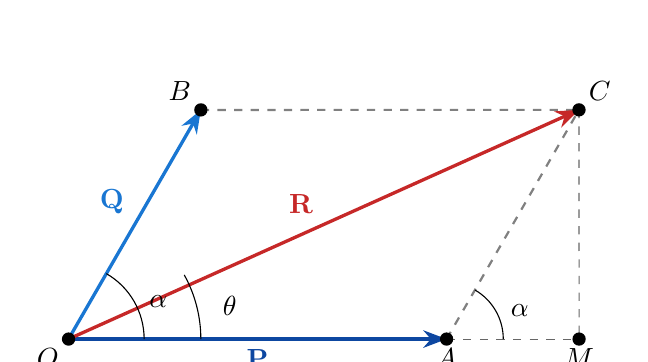
\begin{tikzpicture}[scale=1.2, >=Stealth]
    % Coordinates
    \coordinate (O) at (0,0);
    \coordinate (P) at (4,0);
    \coordinate (Q) at (60:2.8);
    \coordinate (R) at ($(P)+(Q)$);
    \coordinate (M) at (R|-O);

    % Parallelogram sides
    \draw[very thick, ->, color=primary] (O) -- (P) node[midway, below] {$\mathbf{P}$};
    \draw[very thick, ->, color=secondary] (O) -- (Q) node[midway, above left] {$\mathbf{Q}$};
    \draw[dashed, thick, color=gray] (P) -- (R);
    \draw[dashed, thick, color=gray] (Q) -- (R);
    \draw[very thick, ->, color=examcolor] (O) -- (R) node[midway, above left] {$\mathbf{R}$};
    \draw[dashed, color=black!60] (R) -- (M);
    \draw[dashed, color=black!60] (P) -- (M);

    % Nodes
    \fill (O) circle (2pt) node[below left] {$O$};
    \fill (P) circle (2pt) node[below] {$A$};
    \fill (Q) circle (2pt) node[above left] {$B$};
    \fill (R) circle (2pt) node[above right] {$C$};
    \fill (M) circle (2pt) node[below] {$M$};

    % Angles
    \draw (0.8,0) arc (0:60:0.8) node[midway, right=2pt] {$\alpha$};
    \draw (1.4,0) arc (0:29:1.4) node[midway, right=6pt] {$\theta$};
    \draw (P) +(0.6,0) arc (0:60:0.6) node[midway, right=2pt] {$\alpha$};
\end{tikzpicture}
\end{center}

\begin{proofbox}{Derivation of Resultant Magnitude and Direction}
Let two forces $P$ and $Q$ act at point $O$ at an angle $\alpha$ to each other. Let $OA = P$ and $OB = Q$. Complete the parallelogram $OACB$. The diagonal $OC = R$ represents the resultant force.

From vertex $C$, drop a perpendicular $CM$ onto the extension of $OA$.
In right-angled triangle $\triangle PCM$:
\[
PM = AC \cos\alpha = Q \cos\alpha, \quad CM = AC \sin\alpha = Q \sin\alpha
\]
Total horizontal length $OM$:
\[
OM = OA + PM = P + Q \cos\alpha
\]
In right-angled triangle $\triangle OCM$, by Pythagoras' Theorem:
\[
OC^2 = OM^2 + CM^2 = (P + Q \cos\alpha)^2 + (Q \sin\alpha)^2
\]
Expanding the square:
\[
R^2 = P^2 + 2PQ \cos\alpha + Q^2 \cos^2\alpha + Q^2 \sin^2\alpha = P^2 + Q^2 + 2PQ \cos\alpha
\]
Taking the square root gives the **Magnitude of Resultant**:
\begin{equation}
R = \sqrt{P^2 + Q^2 + 2PQ \cos\alpha}
\end{equation}

Let $\theta$ be the angle made by resultant $R$ with force $P$. From $\triangle OCM$:
\begin{equation}
\tan\theta = \frac{CM}{OM} = \frac{Q \sin\alpha}{P + Q \cos\alpha}
\end{equation}

\textbf{Special Cases}:
\begin{enumerate}
    \item When $\alpha = 0^\circ$ (forces in same direction): $R = P + Q$, $\theta = 0^\circ$.
    \item When $\alpha = 90^\circ$ (forces perpendicular): $R = \sqrt{P^2 + Q^2}$, $\tan\theta = Q / P$.
    \item When $\alpha = 180^\circ$ (forces in opposite direction): $R = |P - Q|$.
\end{enumerate}
\end{proofbox}

\subsection{Triangle and Polygon Laws of Forces}

\begin{theorembox}{Triangle Law of Forces}
If three forces acting on a particle can be represented in magnitude and direction by the three sides of a triangle taken in order, then the particle is in \textbf{static equilibrium}.
\end{theorembox}

\begin{theorembox}{Polygon Law of Forces}
If any number of coplanar forces acting at a point can be represented in magnitude and direction by the sides of a closed polygon taken in order, their resultant is zero and the forces are in equilibrium.
\end{theorembox}

\subsection{Analytical Method of Resolution for Coplanar Concurrent Forces}
When a system of $n$ coplanar concurrent forces $F_1, F_2, \dots, F_n$ acts at a point $O$ making angles $\theta_1, \theta_2, \dots, \theta_n$ with a horizontal $X$-axis:
\begin{enumerate}
    \item Sum of components along $X$-axis: $X = \sum_{i=1}^n F_i \cos\theta_i$
    \item Sum of components along $Y$-axis: $Y = \sum_{i=1}^n F_i \sin\theta_i$
    \item Resultant magnitude: $R = \sqrt{X^2 + Y^2}$
    \item Direction angle with $X$-axis: $\theta = \tan^{-1}\left(\frac{Y}{X}\right)$
\end{enumerate}

\begin{importantbox}{Conditions of Equilibrium for Coplanar Concurrent Forces}
For a particle under coplanar concurrent forces to be in static equilibrium ($R = 0$):
\begin{equation}
\sum X = 0 \quad \text{and} \quad \sum Y = 0
\end{equation}
\end{importantbox}

\subsection{Lami's Theorem}

\begin{theorembox}{Lami's Theorem}
If three coplanar concurrent forces acting at a point are in equilibrium, then each force is proportional to the sine of the angle between the other two forces.
\end{theorembox}

\begin{center}
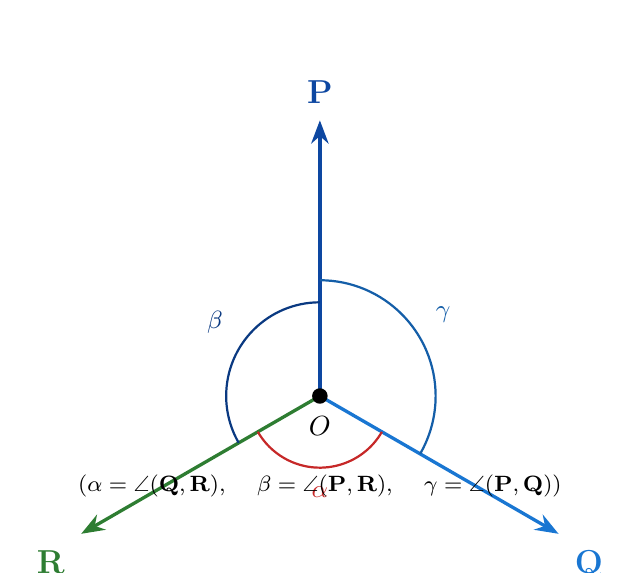
\begin{tikzpicture}[scale=1.4, >=Stealth]
    % Origin
    \coordinate (O) at (0,0);
    \coordinate (P) at (90:2.5);
    \coordinate (Q) at (-30:2.5);
    \coordinate (R) at (210:2.5);

    % Force vectors
    \draw[very thick, ->, color=primary] (O) -- (P) node[above=2pt, font=\large\bfseries] {$\mathbf{P}$};
    \draw[very thick, ->, color=secondary] (O) -- (Q) node[below right=2pt, font=\large\bfseries] {$\mathbf{Q}$};
    \draw[very thick, ->, color=proofcolor] (O) -- (R) node[below left=2pt, font=\large\bfseries] {$\mathbf{R}$};

    \fill (O) circle (2pt) node[below=4pt] {$O$};

    % Distinct angle arcs with no text overlap
    \draw[thick, color=examcolor] (-30:0.65) arc (-30:-150:0.65) node[midway, below=3pt, font=\small\bfseries] {$\alpha$};
    \draw[thick, color=primary!80!black] (90:0.85) arc (90:210:0.85) node[midway, above left=2pt, font=\small\bfseries] {$\beta$};
    \draw[thick, color=secondary!80!black] (90:1.05) arc (90:-30:1.05) node[midway, above right=2pt, font=\small\bfseries] {$\gamma$};
    
    % Legend annotation below diagram
    \node[below=25pt] at (O) {\footnotesize ($\alpha = \angle(\mathbf{Q},\mathbf{R})$, \quad $\beta = \angle(\mathbf{P},\mathbf{R})$, \quad $\gamma = \angle(\mathbf{P},\mathbf{Q})$)};
\end{tikzpicture}
\end{center}

\begin{proofbox}{Rigorous Proof of Lami's Theorem}
Let three forces $\mathbf{P}, \mathbf{Q}, \mathbf{R}$ act at point $O$ in equilibrium. Let:
- $\alpha$ be the angle between $\mathbf{Q}$ and $\mathbf{R}$
- $\beta$ be the angle between $\mathbf{P}$ and $\mathbf{R}$
- $\gamma$ be the angle between $\mathbf{P}$ and $\mathbf{Q}$

Since the forces are in equilibrium, by the Triangle Law of Forces, they can be represented by the sides $AB, BC, CA$ of a closed triangle $\triangle ABC$ taken in order, where $AB = P$, $BC = Q$, $CA = R$.

\begin{center}
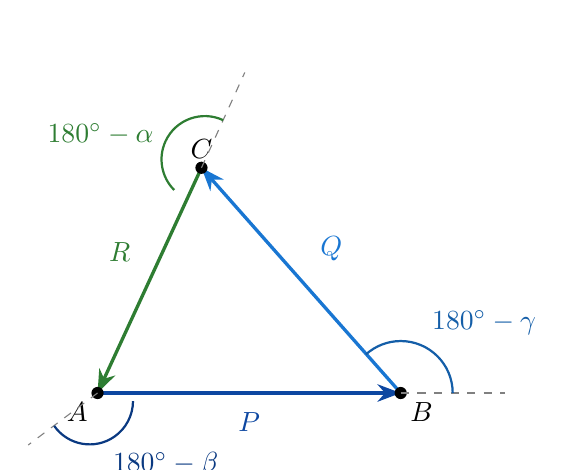
\begin{tikzpicture}[scale=1.1, >=Stealth]
    \coordinate (A) at (0,0);
    \coordinate (B) at (3.5,0);
    \coordinate (C) at (1.2,2.6);

    \draw[very thick, ->, color=primary] (A) -- (B) node[midway, below=3pt, font=\bfseries] {$P$};
    \draw[very thick, ->, color=secondary] (B) -- (C) node[midway, above right=3pt, font=\bfseries] {$Q$};
    \draw[very thick, ->, color=proofcolor] (C) -- (A) node[midway, above left=3pt, font=\bfseries] {$R$};

    \fill (A) circle (2pt) node[below left] {$A$};
    \fill (B) circle (2pt) node[below right] {$B$};
    \fill (C) circle (2pt) node[above] {$C$};

    % Extended lines for exterior angles
    \draw[dashed, gray] (B) -- +(1.2,0);
    \draw[dashed, gray] (C) -- +(0.5,1.1);
    \draw[dashed, gray] (A) -- +(-0.8,-0.6);

    % Exterior angle arcs
    \draw[thick, color=secondary!80!black] (B) +(0.6,0) arc (0:132:0.6) node[midway, above right] {$180^\circ - \gamma$};
    \draw[thick, color=proofcolor] (C) +(0.25,0.55) arc (65:225:0.5) node[midway, left=2pt] {$180^\circ - \alpha$};
    \draw[thick, color=primary!80!black] (A) +(-0.5,-0.38) arc (215:360:0.5) node[midway, below right] {$180^\circ - \beta$};
\end{tikzpicture}
\end{center}

The interior angles of triangle $\triangle ABC$ are given by:
\[
\angle A = 180^\circ - \alpha, \quad \angle B = 180^\circ - \beta, \quad \angle C = 180^\circ - \gamma
\]
Applying the **Sine Rule** to $\triangle ABC$:
\[
\frac{AB}{\sin\angle C} = \frac{BC}{\sin\angle A} = \frac{CA}{\sin\angle B}
\]
Substituting the force magnitudes and angles:
\[
\frac{P}{\sin(180^\circ - \alpha)} = \frac{Q}{\sin(180^\circ - \beta)} = \frac{R}{\sin(180^\circ - \gamma)}
\]
Since $\sin(180^\circ - x) = \sin x$, we obtain Lami's Formula:
\begin{equation}
\frac{P}{\sin\alpha} = \frac{Q}{\sin\beta} = \frac{R}{\sin\gamma}
\end{equation}
\end{proofbox}

\subsection{Solved Examples on Coplanar Concurrent Forces}

\begin{examplebox}{Three Equal Angles in Lami's Theorem}
Three coplanar concurrent forces $P, Q, R$ act at a point $O$ in equilibrium. If the angles between any pair of forces are equal to $120^\circ$, show that $P = Q = R$.
\end{examplebox}

\begin{proofbox}{Solution}
Given $\alpha = \beta = \gamma = 120^\circ$. Applying Lami's Theorem:
\[
\frac{P}{\sin 120^\circ} = \frac{Q}{\sin 120^\circ} = \frac{R}{\sin 120^\circ}
\]
Since $\sin 120^\circ = \sqrt{3}/2 \neq 0$, multiplying by $\sin 120^\circ$ yields:
\begin{equation}
P = Q = R
\end{equation}
\end{proofbox}

\begin{examplebox}{Sphere Resting Between Two Smooth Inclined Planes}
A smooth sphere of weight $W$ and radius $r$ rests between two smooth inclined planes making angles $\alpha$ and $\beta$ with the horizontal. Find the normal reactions exerted by the planes on the sphere.
\end{examplebox}

\begin{center}
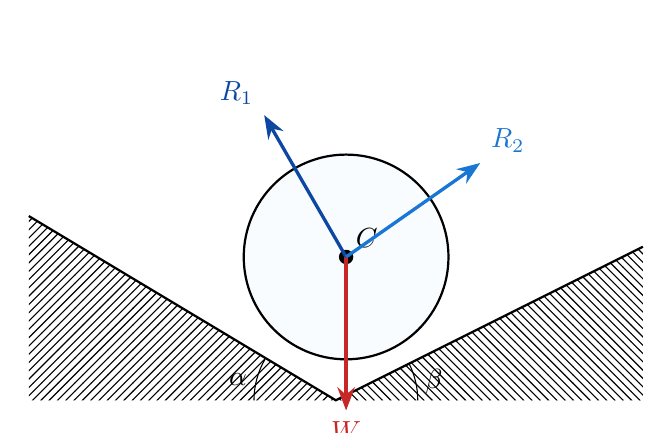
\begin{tikzpicture}[scale=1.3, >=Stealth]
    % Inclined planes
    \draw[thick] (-3,1.8) -- (0,0) -- (3,1.5);
    \fill[pattern=north east lines] (-3,1.8) -- (0,0) -- (-3,0) -- cycle;
    \fill[pattern=north west lines] (3,1.5) -- (0,0) -- (3,0) -- cycle;

    % Angle arcs at base
    \draw (-0.8,0) arc (180:150:0.8) node[midway, left] {$\alpha$};
    \draw (0.8,0) arc (0:26.5:0.8) node[midway, right] {$\beta$};

    % Sphere
    \coordinate (C) at (0.1, 1.4);
    \draw[thick, fill=accent!20] (C) circle (1.0);
    \fill (C) circle (2pt) node[above right] {$C$};

    % Forces acting at C
    \draw[very thick, ->, color=examcolor] (C) -- +(0,-1.5) node[below] {$W$};
    \draw[very thick, ->, color=primary] (C) -- +(120:1.6) node[above left] {$R_1$};
    \draw[very thick, ->, color=secondary] (C) -- +(35:1.6) node[above right] {$R_2$};
\end{tikzpicture}
\end{center}

\begin{proofbox}{Solution}
Three forces act on the sphere in equilibrium at its center $C$:
1. Weight $W$ acting vertically downwards.
2. Normal reaction $R_1$ perpendicular to the first plane (inclined at angle $90^\circ - \alpha$ to horizontal).
3. Normal reaction $R_2$ perpendicular to the second plane (inclined at angle $90^\circ - \beta$ to horizontal).

The angles between the force vectors are:
- Angle between $R_1$ and $R_2 = 180^\circ - (\alpha + \beta)$
- Angle between $R_1$ and $W = 180^\circ - \alpha$
- Angle between $R_2$ and $W = 180^\circ - \beta$

Applying **Lami's Theorem** at center $C$:
\[
\frac{W}{\sin[180^\circ - (\alpha + \beta)]} = \frac{R_1}{\sin(180^\circ - \beta)} = \frac{R_2}{\sin(180^\circ - \alpha)}
\]
Using $\sin(180^\circ - x) = \sin x$:
\[
\frac{W}{\sin(\alpha + \beta)} = \frac{R_1}{\sin\beta} = \frac{R_2}{\sin\alpha}
\]
Solving for the normal reactions:
\begin{equation}
R_1 = \frac{W \sin\beta}{\sin(\alpha + \beta)}, \qquad R_2 = \frac{W \sin\alpha}{\sin(\alpha + \beta)}
\end{equation}
\end{proofbox}

\begin{examplebox}{Particle Suspended by Strings}
A particle of weight $W$ is suspended from two fixed points $A$ and $B$ in the same horizontal line by two light inextensible strings $AC$ and $BC$ of lengths $a$ and $b$ respectively. If the distance $AB = c$, find the tensions $T_1$ and $T_2$ in the strings.
\end{examplebox}

\begin{proofbox}{Solution}
Let $\angle CAB = A$ and $\angle CBA = B$. The string angles with the vertical line at $C$ are $90^\circ - A$ and $90^\circ - B$.
The three concurrent forces at $C$ are $T_1$ along $CA$, $T_2$ along $CB$, and weight $W$ vertically downwards.

Applying Lami's Theorem at $C$:
\[
\frac{T_1}{\sin(90^\circ + B)} = \frac{T_2}{\sin(90^\circ + A)} = \frac{W}{\sin(180^\circ - A - B)}
\]
Since $\sin(90^\circ + x) = \cos x$ and $\sin(A+B) = \sin C$:
\[
\frac{T_1}{\cos B} = \frac{T_2}{\cos A} = \frac{W}{\sin C}
\]
Thus:
\begin{equation}
T_1 = \frac{W \cos B}{\sin C}, \qquad T_2 = \frac{W \cos A}{\sin C}
\end{equation}
Using standard triangle relations $c = a \cos B + b \cos A$ and $\sin C = \frac{c}{2R}$, we can write $T_1$ and $T_2$ purely in terms of side lengths $a, b, c$.
\end{proofbox}

% =========================================================================
\section{Unit 2: Moments, Parallel Forces, and Couples}
% =========================================================================

\subsection{Moment of a Force}

\begin{definitionbox}{Moment of a Force about a Point}
The \textbf{moment of a force} $\mathbf{F}$ about a point $O$ measures the turning or rotational effect of the force about $O$.
Mathematically, the moment vector $\mathbf{M}_O$ is defined as:
\begin{equation}
\mathbf{M}_O = \mathbf{r} \times \mathbf{F}
\end{equation}
where $\mathbf{r}$ is the position vector of any point on the line of action of $\mathbf{F}$ relative to $O$.

Scalar magnitude of moment:
\begin{equation}
M = F \cdot p
\end{equation}
where $p$ is the perpendicular distance from $O$ to the line of action of $\mathbf{F}$.
\end{definitionbox}

\begin{theorembox}{Geometrical Representation of Moment}
The magnitude of the moment of a force represented by vector $\mathbf{AB}$ about a point $O$ is equal to **twice the area** of the triangle $\triangle OAB$.
\end{theorembox}

\subsection{Varignon's Theorem of Moments}

\begin{theorembox}{Varignon's Theorem of Moments}
The algebraic sum of the moments of any two coplanar forces about any point in their plane is equal to the moment of their resultant about that same point.
\end{theorembox}

\begin{center}
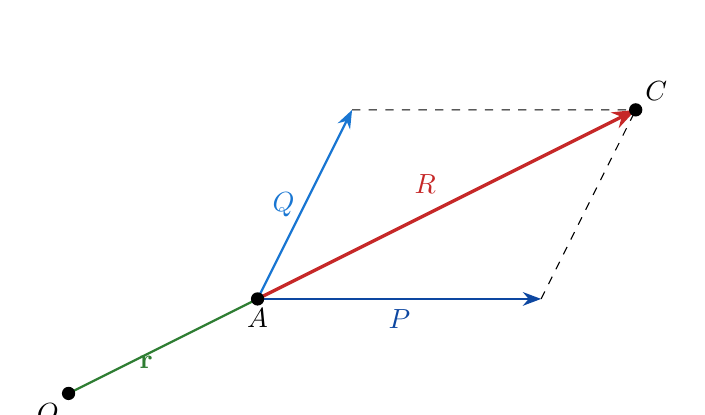
\begin{tikzpicture}[scale=1.2, >=Stealth]
    % Origin of moment O
    \coordinate (O) at (0,0);
    \coordinate (A) at (2,1);
    \coordinate (P) at (5,1);
    \coordinate (Q) at (3,3);
    \coordinate (R) at ($(P)+(Q)-(A)$);

    \draw[thick, ->, color=primary] (A) -- (P) node[midway, below] {$P$};
    \draw[thick, ->, color=secondary] (A) -- (Q) node[midway, left] {$Q$};
    \draw[very thick, ->, color=examcolor] (A) -- (R) node[midway, above left] {$R$};

    \draw[dashed] (P) -- (R);
    \draw[dashed] (Q) -- (R);

    % Lines to O
    \draw[thick, color=proofcolor] (O) -- (A) node[midway, below left] {$\mathbf{r}$};
    \fill (O) circle (2pt) node[below left] {$O$};
    \fill (A) circle (2pt) node[below] {$A$};
    \fill (R) circle (2pt) node[above right] {$C$};
\end{tikzpicture}
\end{center}

\begin{proofbox}{Proof 1: Vector Proof of Varignon's Theorem}
Let two forces $\mathbf{P}$ and $\mathbf{Q}$ act at point $A$ with position vector $\mathbf{r}$ relative to moment center $O$.
The resultant force $\mathbf{R}$ is:
\[
\mathbf{R} = \mathbf{P} + \mathbf{Q}
\]
Taking the vector cross product with $\mathbf{r}$ from the left:
\[
\mathbf{r} \times \mathbf{R} = \mathbf{r} \times (\mathbf{P} + \mathbf{Q})
\]
Using the distributive property of vector cross product:
\begin{equation}
\mathbf{r} \times \mathbf{R} = (\mathbf{r} \times \mathbf{P}) + (\mathbf{r} \times \mathbf{Q})
\end{equation}
Thus, the vector moment of resultant $\mathbf{R}$ about $O$ equals the sum of vector moments of $\mathbf{P}$ and $\mathbf{Q}$ about $O$.

Taking the scalar projection perpendicular to the plane yields the scalar Varignon's Theorem:
\begin{equation}
M_O(R) = M_O(P) + M_O(Q)
\end{equation}
\end{proofbox}

\begin{proofbox}{Proof 2: Varignon's Theorem for Parallel Forces}
Let two like parallel forces $P$ and $Q$ act at points $A$ and $B$. Their resultant $R = P + Q$ acts at point $C$ on line $AB$ such that $P \cdot AC = Q \cdot CB$.
Take any point $O$ on the line $AB$ extended beyond $A$.

Taking moments about $O$:
- Moment of $P$ about $O = P \cdot OA$
- Moment of $Q$ about $O = Q \cdot OB = Q (OA + AB) = Q \cdot OA + Q \cdot AB$

Sum of moments of $P$ and $Q$ about $O$:
\[
M_O(P) + M_O(Q) = P \cdot OA + Q \cdot OA + Q \cdot AB = (P + Q) OA + Q \cdot AB
\]
Since $P \cdot AC = Q \cdot CB = Q (AB - AC) \implies (P+Q) AC = Q \cdot AB$, we substitute $Q \cdot AB = (P+Q) AC$:
\[
M_O(P) + M_O(Q) = (P + Q) OA + (P + Q) AC = (P + Q) (OA + AC) = (P + Q) OC = R \cdot OC
\]
This equals the moment of resultant $R = P + Q$ about $O$. Thus Varignon's Theorem holds for parallel forces as well.
\end{proofbox}

\subsection{Parallel Forces and Center of Parallel Forces}

\begin{definitionbox}{Like and Unlike Parallel Forces}
1. \textbf{Like Parallel Forces}: Forces whose lines of action are parallel and act in the **same direction**.
2. \textbf{Unlike Parallel Forces}: Forces whose lines of action are parallel but act in **opposite directions**.
\end{definitionbox}

\begin{proofbox}{Resultant of Like Parallel Forces}
Let two like parallel forces $P$ and $Q$ act at points $A$ and $B$ separated by distance $d$.
1. **Magnitude of Resultant**: $R = P + Q$ acting in the same parallel direction.
2. **Line of Action**: Resultant $R$ acts at a point $C$ on segment $AB$ such that:
\begin{equation}
P \cdot AC = Q \cdot CB \implies \frac{AC}{CB} = \frac{Q}{P}
\end{equation}
Thus, $C$ divides $AB$ internally in the inverse ratio of the forces.
\end{proofbox}

\begin{proofbox}{Resultant of Unlike Parallel Forces}
Let two unequal unlike parallel forces $P$ and $Q$ ($P > Q$) act at $A$ and $B$.
1. **Magnitude of Resultant**: $R = P - Q$ acting in the direction of the larger force $P$.
2. **Line of Action**: Resultant $R$ acts at a point $C$ on the extension of line $AB$ beyond $A$ such that:
\begin{equation}
P \cdot AC = Q \cdot BC
\end{equation}
Thus, $C$ divides $AB$ externally in the inverse ratio of the forces.
\end{proofbox}

\subsection{Couples and Properties of Couples}

\begin{definitionbox}{Couple and Moment of a Couple}
A \textbf{couple} consists of two equal, opposite, and non-collinear parallel forces $(P, -P)$.

- The perpendicular distance $d$ between their lines of action is called the **arm of the couple**.
- The **moment of the couple** $G$ is the product of force magnitude $P$ and arm $d$:
\begin{equation}
G = P \cdot d
\end{equation}
\end{definitionbox}

\begin{importantbox}{Key Properties of Couples}
1. The vector sum of forces in a couple is zero ($\sum \mathbf{F} = \mathbf{0}$). A couple produces **pure rotation** without translation.
2. The algebraic sum of moments of forces of a couple about ANY point in its plane is **constant** and equal to $P \cdot d$.
3. Two couples in the same plane are **equivalent** if and only if their moments are equal in magnitude and sign.
\end{importantbox}

\subsection{Solved Examples on Moments, Parallel Forces and Hexagons}

\begin{examplebox}{Forces Along Sides of a Regular Hexagon}
Forces of magnitudes $P, 2P, 3P, 4P, 5P, 6P$ act along the sides $AB, BC, CD, DE, EF, FA$ of a regular hexagon $ABCDEF$ of side $a$ taken in order. Find the magnitude, direction, and line of action of their resultant.
\end{examplebox}

\begin{proofbox}{Solution}
Let side $AB$ lie along the $X$-axis. The internal angles of a regular hexagon are $120^\circ$, so exterior side inclinations with $X$-axis are $0^\circ, 60^\circ, 120^\circ, 180^\circ, 240^\circ, 300^\circ$.

1. **Sum of Force Components along $X$-axis**:
\[
X = P\cos 0^\circ + 2P\cos 60^\circ + 3P\cos 120^\circ + 4P\cos 180^\circ + 5P\cos 240^\circ + 6P\cos 300^\circ
\]
\[
X = P(1) + 2P\left(\frac{1}{2}\right) + 3P\left(-\frac{1}{2}\right) + 4P(-1) + 5P\left(-\frac{1}{2}\right) + 6P\left(\frac{1}{2}\right) = -3P
\]

2. **Sum of Force Components along $Y$-axis**:
\[
Y = P\sin 0^\circ + 2P\sin 60^\circ + 3P\sin 120^\circ + 4P\sin 180^\circ + 5P\sin 240^\circ + 6P\sin 300^\circ
\]
\[
Y = P(0) + 2P\left(\frac{\sqrt{3}}{2}\right) + 3P\left(\frac{\sqrt{3}}{2}\right) + 4P(0) + 5P\left(-\frac{\sqrt{3}}{2}\right) + 6P\left(-\frac{\sqrt{3}}{2}\right) = -3\sqrt{3}P
\]

3. **Magnitude and Direction of Resultant**:
\begin{equation}
R = \sqrt{X^2 + Y^2} = \sqrt{(-3P)^2 + (-3\sqrt{3}P)^2} = \sqrt{9P^2 + 27P^2} = \sqrt{36P^2} = 6P
\end{equation}
\[
\tan\theta = \frac{Y}{X} = \frac{-3\sqrt{3}P}{-3P} = \sqrt{3} \implies \theta = 240^\circ
\]

4. **Resultant Moment $G$ about Center $O$**:
Distance of center $O$ to any side is $p = a \sin 60^\circ = \frac{\sqrt{3}}{2}a$.
\[
G = (P + 2P + 3P + 4P + 5P + 6P) p = 21 P \left(\frac{\sqrt{3}}{2}a\right) = \frac{21\sqrt{3}}{2} Pa
\]
Line of action is given by $xY - yX = G_O$.
\end{proofbox}

% =========================================================================
\section{Unit 3: General System of Coplanar Forces \& Trigonometric Theorems}
% =========================================================================

\subsection{Reduction of General Coplanar Force System}

\begin{theorembox}{Reduction Theorem}
Any system of coplanar forces acting on a rigid body can be reduced to a single force $R$ acting at an arbitrarily chosen base point $O$, together with a single couple $G$ in the plane.
\end{theorembox}

\begin{proofbox}{Analytical Derivation of Reduction}
Let $n$ coplanar forces $F_1, F_2, \dots, F_n$ act at points $(x_1, y_1), (x_2, y_2), \dots, (x_n, y_n)$ relative to rectangular axes $OXY$.
Let force $F_i$ have components $(X_i, Y_i)$ along $X$ and $Y$ axes.

1. **Transfers to Origin $O$**: Each force component $X_i$ at $(x_i, y_i)$ is equivalent to a force component $X_i$ at origin $O$ plus a couple of moment $-y_i X_i$.
   Each force component $Y_i$ at $(x_i, y_i)$ is equivalent to a force component $Y_i$ at origin $O$ plus a couple of moment $x_i Y_i$.

2. **Summing Force Components at $O$**:
   \begin{equation}
   X = \sum_{i=1}^n X_i, \qquad Y = \sum_{i=1}^n Y_i
   \end{equation}
   Resultant Force Magnitude:
   \begin{equation}
   R = \sqrt{X^2 + Y^2}
   \end{equation}

3. **Summing Moments of Couples**:
   \begin{equation}
   G = \sum_{i=1}^n (x_i Y_i - y_i X_i)
   \end{equation}
\end{proofbox}

\subsection{Change of Base Point and Line of Action}

\begin{proofbox}{Change of Base Point}
If the base point is changed from origin $O(0,0)$ to a new point $O'(a, b)$, the force components $(X, Y)$ remain unchanged, but the couple moment changes to $G'$:
\begin{equation}
G' = G - aY + bX
\end{equation}
\end{proofbox}

\begin{theorembox}{Line of Action of Resultant}
If $R \neq 0$, the resultant couple $G'$ vanishes at a point $(x, y)$ on the line of action of $R$.
Setting $G' = 0$ with $a = x, b = y$ yields the equation of the **Line of Action**:
\begin{equation}
G - xY + yX = 0 \quad \iff \quad xY - yX = G
\end{equation}
\end{theorembox}

\subsection{General Conditions of Equilibrium of Coplanar Forces}

\begin{importantbox}{Three Sets of Equilibrium Conditions}
For a general system of coplanar forces acting on a rigid body to be in static equilibrium:

**Standard Conditions**:
\begin{equation}
X = 0, \qquad Y = 0, \qquad G = 0
\end{equation}

**Three-Point Moment Conditions**:
The sum of moments about three non-collinear points $A, B, C$ must vanish:
\begin{equation}
M_A = 0, \qquad M_B = 0, \qquad M_C = 0
\end{equation}

**Two-Point Moment Conditions with One Resolution**:
\begin{equation}
M_A = 0, \qquad M_B = 0, \qquad X = 0
\end{equation}
where line $AB$ is not perpendicular to $X$-axis.
\end{importantbox}

\begin{proofbox}{Proof of Three-Point Moment Equilibrium Theorem}
Suppose $M_A = 0, M_B = 0, M_C = 0$ for three non-collinear points $A, B, C$.
If the system reduces to a single resultant force $R$, then:
- $M_A = 0 \implies$ line of action of $R$ passes through $A$.
- $M_B = 0 \implies$ line of action of $R$ passes through $B$.
- $M_C = 0 \implies$ line of action of $R$ passes through $C$.

Since $A, B, C$ form a non-degenerate triangle, no single straight line can pass through all three points simultaneously unless $R = 0$.
If the system reduces to a couple $G$, then $M_A = M_B = M_C = G = 0$.
Hence $R = 0$ and $G = 0$, which proves that the system is in static equilibrium.
\end{proofbox}

\subsection{The Trigonometric $m-n$ Theorem for Triangles}

\begin{theorembox}{The $m-n$ Theorem}
Let $CD$ be a line segment drawn from vertex $C$ of triangle $\triangle ABC$ to base $AB$, dividing $AB$ into two segments $AD$ and $DB$ such that $AD : DB = m : n$. Let $\angle CDB = \theta$.
\begin{enumerate}
    \item If $CD$ divides $\angle C$ into angles $\alpha$ ($\angle ACD$) and $\beta$ ($\angle BCD$):
    \begin{equation}
    (m + n) \cot\theta = m \cot\alpha - n \cot\beta
    \end{equation}
    \item If angles at base are $A$ and $B$:
    \begin{equation}
    (m + n) \cot\theta = n \cot A - m \cot B
    \end{equation}
\end{enumerate}
\end{theorembox}

\begin{center}
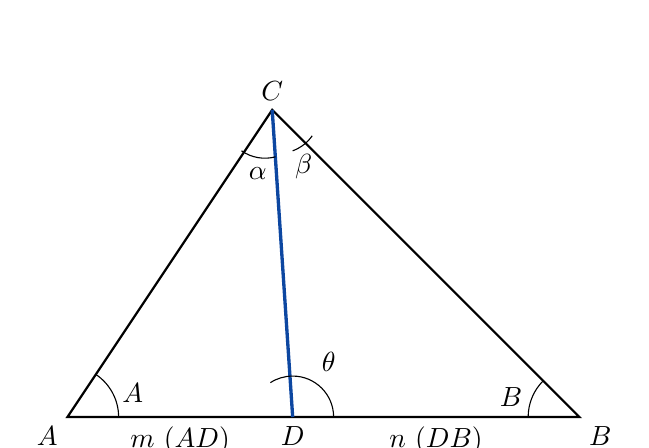
\begin{tikzpicture}[scale=1.3, >=Stealth]
    \coordinate (A) at (0,0);
    \coordinate (B) at (5,0);
    \coordinate (C) at (2,3);
    \coordinate (D) at (2.2,0);

    \draw[thick] (A) -- (B) -- (C) -- cycle;
    \draw[very thick, color=primary] (C) -- (D);

    % Segment lengths
    \node[below] at ($(A)!0.5!(D)$) {$m$ ($AD$)};
    \node[below] at ($(D)!0.5!(B)$) {$n$ ($DB$)};

    % Labels
    \node[below left] at (A) {$A$};
    \node[below right] at (B) {$B$};
    \node[above] at (C) {$C$};
    \node[below] at (D) {$D$};

    % Angles
    \draw (D) +(0.4,0) arc (0:123:0.4) node[midway, above right] {$\theta$};
    \draw (A) +(0.5,0) arc (0:56:0.5) node[midway, right] {$A$};
    \draw (B) +(-0.5,0) arc (180:135:0.5) node[midway, left] {$B$};
    \draw (C) +(-0.3,-0.4) arc (235:285:0.4) node[midway, below] {$\alpha$};
    \draw (C) +(0.2,-0.4) arc (290:325:0.4) node[midway, below] {$\beta$};
\end{tikzpicture}
\end{center}

\begin{proofbox}{Rigorous Proof of $m-n$ Theorem}
In $\triangle ACD$, applying Sine Rule:
\[
\frac{AD}{\sin\alpha} = \frac{CD}{\sin A} \implies AD = CD \frac{\sin\alpha}{\sin A}
\]
Since $\angle ADC = 180^\circ - \theta$, $\angle ACD = \alpha$, so $A = \theta - \alpha$.
Thus $AD = CD \frac{\sin\alpha}{\sin(\theta - \alpha)}$.

In $\triangle BCD$, applying Sine Rule:
\[
\frac{DB}{\sin\beta} = \frac{CD}{\sin B} \implies DB = CD \frac{\sin\beta}{\sin B}
\]
Since $\angle BDC = \theta$, $\angle BCD = \beta$, so $B = 180^\circ - (\theta + \beta)$, $\sin B = \sin(\theta + \beta)$.
Thus $DB = CD \frac{\sin\beta}{\sin(\theta + \beta)}$.

Taking the ratio $AD / DB = m / n$:
\[
\frac{m}{n} = \frac{\sin\alpha}{\sin(\theta - \alpha)} \cdot \frac{\sin(\theta + \beta)}{\sin\beta} = \frac{\sin\alpha(\sin\theta\cos\beta + \cos\theta\sin\beta)}{\sin\beta(\sin\theta\cos\alpha - \cos\theta\sin\alpha)}
\]
Dividing numerator and denominator by $\sin\theta \sin\alpha \sin\beta$:
\[
\frac{m}{n} = \frac{\cot\beta + \cot\theta}{\cot\alpha - \cot\theta}
\]
Cross-multiplying:
\[
m(\cot\alpha - \cot\theta) = n(\cot\beta + \cot\theta)
\]
Rearranging terms:
\[
m\cot\alpha - n\cot\beta = (m+n)\cot\theta
\]
This proves Part 1. Part 2 is proved similarly using base angles $A$ and $B$.
\end{proofbox}

\subsection{Solved Examples on Triangle Force Centers \& $m-n$ Theorem}

\begin{examplebox}{Resultant Passing Through Triangle Special Points}
Three forces $P, Q, R$ act along sides $BC, CA, AB$ of $\triangle ABC$. Show that the resultant passes through:
1. **Incenter $I$**: $P + Q + R = 0$
2. **Circumcenter $O$**: $P\cos A + Q\cos B + R\cos C = 0$
3. **Orthocenter $H$**: $P\sec A + Q\sec B + R\sec C = 0$
4. **Centroid $G$**: $Pa + Qb + Rc = 0$ (or $P\csc A + Q\csc B + R\csc C = 0$)
\end{examplebox}

\begin{proofbox}{Solution}
By Varignon's Theorem, if resultant passes through a point $K$, the sum of moments of $P, Q, R$ about $K$ must vanish ($\sum M_K = 0$).

1. **Incenter $I$**: Perpendicular distance to all sides is $r$.
   \[ M_I = P \cdot r + Q \cdot r + R \cdot r = r(P+Q+R) = 0 \implies P+Q+R=0 \]

2. **Circumcenter $O$**: Distance to side $BC$ is $R\cos A$, to $CA$ is $R\cos B$, to $AB$ is $R\cos C$.
   \[ M_O = P(R\cos A) + Q(R\cos B) + R(R\cos C) = R(P\cos A + Q\cos B + R\cos C) = 0 \]
   \[ \implies P\cos A + Q\cos B + R\cos C = 0 \]

3. **Orthocenter $H$**: Perpendicular distance to $BC$ is $2R\cos B \cos C$. Expressing in terms of secants yields:
   \[ P\sec A + Q\sec B + R\sec C = 0 \]

4. **Centroid $G$**: Perpendicular distance to side $BC$ is $\frac{1}{3} h_a = \frac{2\Delta}{3a}$.
   \[ M_G = P\left(\frac{2\Delta}{3a}\right) + Q\left(\frac{2\Delta}{3b}\right) + R\left(\frac{2\Delta}{3c}\right) = \frac{2\Delta}{3}\left(\frac{P}{a} + \frac{Q}{b} + \frac{R}{c}\right) = 0 \]
   Using $a = 2R\sin A$, this simplifies to $P\csc A + Q\csc B + R\csc C = 0$.
\end{proofbox}

\begin{examplebox}{Heavy Uniform Beam on Smooth Inclined Planes}
A uniform beam $AB$ of weight $W$ rests with its ends $A$ and $B$ on two smooth inclined planes of inclinations $\alpha$ and $\beta$ to the horizontal. Find the inclination $\theta$ of the beam to the horizontal in equilibrium.
\end{examplebox}

\begin{proofbox}{Solution}
Let $G$ be the midpoint of uniform beam $AB$ ($AG = GB = a$, so $m=1, n=1$).
The normal reactions $R_1$ at $A$ and $R_2$ at $B$ act at angles $(90^\circ - \alpha)$ and $(90^\circ - \beta)$ to horizontal.
Line of action of weight $W$ is vertical through center of gravity $G$.

Applying Part 2 of $m-n$ Theorem to $\triangle AGB$ with vertical line $GG'$ making angle $90^\circ - \theta$ with beam $AB$:
\[
(1 + 1) \cot(90^\circ - \theta) = 1 \cdot \cot(90^\circ - \alpha) - 1 \cdot \cot(90^\circ - \beta)
\]
Since $\cot(90^\circ - x) = \tan x$:
\[
2 \tan\theta = \tan\alpha - \tan\beta
\]
\begin{equation}
\tan\theta = \frac{1}{2} (\tan\alpha - \tan\beta)
\end{equation}
\end{proofbox}

% =========================================================================
\section{Unit 4: Principle of Virtual Work \& Stability Criteria}
% =========================================================================

\subsection{Virtual Displacement and Virtual Work}

\begin{definitionbox}{Virtual Displacement and Virtual Work}
1. \textbf{Virtual Displacement}: An imaginary, infinitesimal displacement $\delta \mathbf{r}$ of a system of particles consistent with the geometrical constraints, assumed to occur in zero time interval.
2. \textbf{Virtual Work}: The work done by a force $\mathbf{F}$ during a virtual displacement $\delta \mathbf{r}$:
\begin{equation}
\delta W = \mathbf{F} \cdot \delta \mathbf{r} = F_x \delta x + F_y \delta y + F_z \delta z
\end{equation}
\end{definitionbox}

\subsection{Work Done by Common Forces and Constraints}

\begin{theorembox}{Virtual Work done by Internal Constraints}
For ideal workless constraints, the total virtual work done by constraint forces vanishes:
\begin{enumerate}
    \item \textbf{Tension in Light String}: For an inextensible string of length $s$, $\delta W = -T \delta s = 0$.
    \item \textbf{Thrust in Light Rod}: For a rod of constant length $l$, $\delta W = -R \delta l = 0$.
    \item \textbf{Reaction of Smooth Surface}: Normal reaction $N \perp \delta \mathbf{r} \implies \delta W = N \cdot 0 = 0$.
    \item \textbf{Reaction at Fixed Smooth Hinge}: Displacement of point of contact is zero $\implies \delta W = 0$.
    \item \textbf{Gravity Force on Body}: $\delta W = -W \delta y_{cg}$ where $y_{cg}$ is vertical height of center of gravity.
\end{enumerate}
\end{theorembox}

\subsection{Principle of Virtual Work for Coplanar Forces}

\begin{theorembox}{Principle of Virtual Work}
A system of coplanar forces acting on a rigid body or interconnected system of bodies with ideal workless constraints is in **static equilibrium** if and only if the total virtual work done by all external forces in any arbitrary virtual displacement consistent with constraints is zero:
\begin{equation}
\sum \delta W = 0
\end{equation}
\end{theorembox}

\begin{proofbox}{Proof of Principle of Virtual Work}
Consider a system of particles in equilibrium under external forces $\mathbf{F}_i^{(e)}$ and constraint forces $\mathbf{f}_i$.
For each particle $i$ in equilibrium:
\[
\mathbf{F}_i^{(e)} + \mathbf{f}_i = \mathbf{0}
\]
Taking dot product with an arbitrary virtual displacement $\delta \mathbf{r}_i$ and summing over all particles:
\[
\sum_{i} (\mathbf{F}_i^{(e)} + \mathbf{f}_i) \cdot \delta \mathbf{r}_i = 0
\]
\[
\sum_{i} \mathbf{F}_i^{(e)} \cdot \delta \mathbf{r}_i + \sum_{i} \mathbf{f}_i \cdot \delta \mathbf{r}_i = 0
\]
For ideal constraints (fixed hinges, rigid rods, inextensible strings, smooth contacts), the net virtual work done by constraint forces is zero:
\[
\sum_{i} \mathbf{f}_i \cdot \delta \mathbf{r}_i = 0
\]
Therefore, the necessary and sufficient condition for equilibrium is:
\begin{equation}
\sum_{i} \mathbf{F}_i^{(e)} \cdot \delta \mathbf{r}_i = 0 \iff \sum \delta W = 0
\end{equation}
\end{proofbox}

\subsection{Stability of Equilibrium and Potential Energy Criteria}

\begin{definitionbox}{Potential Energy Criterion for Stability}
If all external forces acting on a system are conservative, there exists a potential energy function $V(\theta)$ depending on a single position coordinate $\theta$.
1. **Equilibrium Condition**:
   \begin{equation}
   \frac{dV}{d\theta} = 0
   \end{equation}
2. **Stable Equilibrium**: $V(\theta)$ is at a local **minimum**:
   \begin{equation}
   \frac{d^2 V}{d\theta^2} > 0
   \end{equation}
3. **Unstable Equilibrium**: $V(\theta)$ is at a local **maximum**:
   \begin{equation}
   \frac{d^2 V}{d\theta^2} < 0
   \end{equation}
\end{definitionbox}

\begin{theorembox}{General Stability Formula for Body Resting on Curved Surface}
If a body of weight $W$ with lower surface of radius of curvature $r$ rests on top of a fixed convex surface of radius of curvature $R$, let $h$ be the height of the center of gravity of the upper body above the contact point.
The equilibrium is **STABLE** if:
\begin{equation}
\frac{1}{h} > \frac{1}{r} + \frac{1}{R}
\end{equation}
and **UNSTABLE** if $\frac{1}{h} < \frac{1}{r} + \frac{1}{R}$.

If the lower surface is flat ($R \to \infty$), the stability condition simplifies to:
\begin{equation}
h < r
\end{equation}
\end{theorembox}

\subsection{Solved Examples on Principle of Virtual Work}

\begin{examplebox}{Jointed Hexagon Framework of Rods}
Six equal heavy uniform rods, each of weight $w$ and length $a$, are freely jointed at their ends to form a regular hexagon $ABCDEF$. The framework is suspended vertically from vertex $A$, and kept in shape by a light horizontal rod joining the midpoints of $AB$ and $AF$. A weight $W$ is attached to the lowest vertex $D$. Find the thrust $T$ in the light horizontal rod using Virtual Work.
\end{examplebox}

\begin{proofbox}{Solution using Virtual Work}
Let $\theta$ be the angle each upper rod $AB, AF$ makes with the vertical diagonal $AD$.
For a regular hexagon in standard vertical suspension, $\theta = 30^\circ$.

1. **Heights of Centers of Mass and Points of Action**:
   - Depth of vertex $D$ below $A$: $y_D = 2a\cos\theta + 2a\cos\theta = 4a\cos\theta$.
   - Depth of center of gravity of the 6 rods: $y_{cg} = 2a\cos\theta$.
   - Length of light rod joining midpoints of $AB$ and $AF$: $x = a\sin\theta$.

2. **Virtual Work Equation**:
   Active forces are weight $W$ at $D$, total weight $6w$ at center of gravity, and thrust $T$ along the horizontal rod:
   \begin{equation}
   \delta W = W \delta y_D + 6w \delta y_{cg} + T \delta x = 0
   \end{equation}

3. **Differentiating Coordinates**:
   - $\delta y_D = \delta(4a\cos\theta) = -4a\sin\theta \, \delta\theta$
   - $\delta y_{cg} = \delta(2a\cos\theta) = -2a\sin\theta \, \delta\theta$
   - $\delta x = \delta(a\sin\theta) = a\cos\theta \, \delta\theta$

4. **Substituting**:
   \[
   W(-4a\sin\theta \, \delta\theta) + 6w(-2a\sin\theta \, \delta\theta) + T(a\cos\theta \, \delta\theta) = 0
   \]
   Dividing by $a\delta\theta$:
   \[
   T\cos\theta = (4W + 12w)\sin\theta \implies T = (4W + 12w)\tan\theta
   \]
   For $\theta = 30^\circ$, $\tan 30^\circ = \frac{1}{\sqrt{3}}$:
   \begin{equation}
   T = \frac{4W + 12w}{\sqrt{3}} = (W + 3w) \frac{4}{\sqrt{3}}
   \end{equation}
\end{proofbox}

\begin{examplebox}{Rhombus Framework of Rods}
Four equal light rods each of length $a$ are freely jointed together to form a rhombus $ABCD$. The framework is suspended vertically from vertex $A$. A weight $W$ is attached at the lowest vertex $C$, and the framework is kept in shape by a light inextensible string joining $B$ and $D$. If $\angle DAB = 2\theta$, find the tension $T$ in string $BD$.
\end{examplebox}

\begin{center}
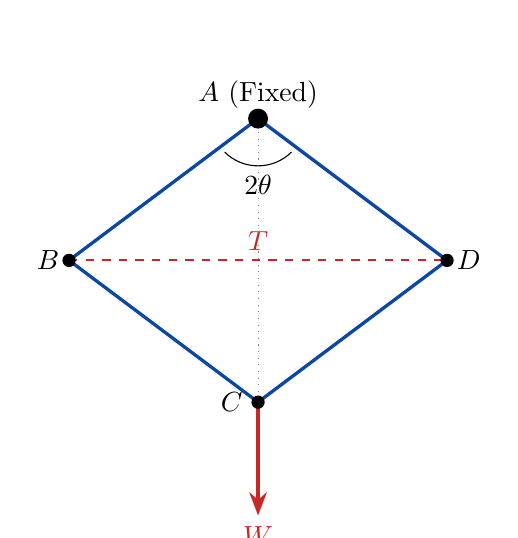
\begin{tikzpicture}[scale=1.2, >=Stealth]
    \coordinate (A) at (0,3);
    \coordinate (B) at (-2,1.5);
    \coordinate (C) at (0,0);
    \coordinate (D) at (2,1.5);

    % Rods
    \draw[very thick, color=primary] (A) -- (B) -- (C) -- (D) -- cycle;
    % String BD
    \draw[thick, dashed, color=examcolor] (B) -- (D) node[midway, above] {$T$};

    % Weight at C
    \draw[very thick, ->, color=examcolor] (C) -- +(0,-1.2) node[below] {$W$};

    % Vertical diagonal AC
    \draw[dotted, color=gray] (A) -- (C);

    % Fixed hinge at A
    \fill (A) circle (3pt) node[above] {$A$ (Fixed)};
    \fill (B) circle (2pt) node[left] {$B$};
    \fill (C) circle (2pt) node[left=2pt] {$C$};
    \fill (D) circle (2pt) node[right] {$D$};

    % Angle at A
    \draw (A) +(225:0.5) arc (225:315:0.5) node[midway, below] {$2\theta$};
\end{tikzpicture}
\end{center}

\begin{proofbox}{Solution using Virtual Work}
Let $A$ be taken as origin $(0,0)$ with $y$-axis vertically downwards.
1. **Coordinates and Lengths**:
   - Distance $AC = 2a \cos\theta$. Depth of weight $W$ from $A$ is $y_C = 2a \cos\theta$.
   - Length of diagonal $BD = 2a \sin\theta = x$.

2. **Virtual Work Equation**:
   The active external forces are weight $W$ at $C$ and tension $T$ along string $BD$.
   \begin{equation}
   \delta W = W \delta y_C - T \delta (BD) = 0
   \end{equation}

3. **Differentiating Coordinates**:
   - $\delta y_C = \delta(2a \cos\theta) = -2a \sin\theta \, \delta\theta$
   - $\delta(BD) = \delta(2a \sin\theta) = 2a \cos\theta \, \delta\theta$

4. **Substituting into Virtual Work Equation**:
   \[
   W (-2a \sin\theta \, \delta\theta) - T (2a \cos\theta \, \delta\theta) = 0
   \]
   Dividing by $-2a \delta\theta$:
   \[
   -W \sin\theta - T \cos\theta = 0 \implies T \cos\theta = -W \sin\theta
   \]
   Taking magnitude of tension:
   \begin{equation}
   T = 2 W \tan\theta
   \end{equation}
\end{proofbox}

\begin{examplebox}{Ladder Leaning against Smooth Wall}
A uniform ladder $AB$ of length $2a$ and weight $W$ rests with its upper end $A$ against a smooth vertical wall and lower end $B$ on a smooth horizontal floor. The ladder is prevented from slipping by a horizontal string connecting $B$ to the corner of the wall and floor. If the ladder makes angle $\theta$ with horizontal, find the tension $T$ in the string using Virtual Work.
\end{examplebox}

\begin{center}
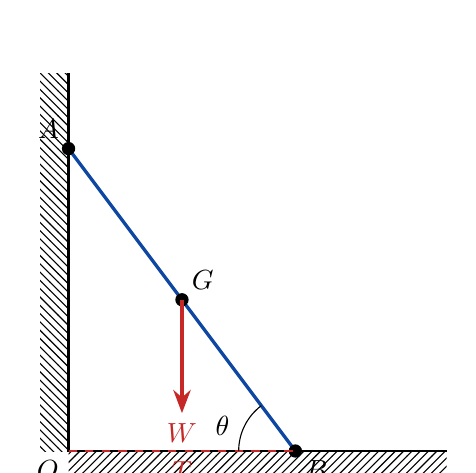
\begin{tikzpicture}[scale=1.2, >=Stealth]
    % Wall and Floor
    \draw[thick] (0,4) -- (0,0) -- (4,0);
    \fill[pattern=north west lines] (-0.3,0) rectangle (0,4);
    \fill[pattern=north east lines] (0,-0.3) rectangle (4,0);

    % Ladder
    \coordinate (A) at (0,3.2);
    \coordinate (B) at (2.4,0);
    \coordinate (G) at ($(A)!0.5!(B)$);

    \draw[very thick, color=primary] (A) -- (B);
    \fill (A) circle (2pt) node[above left] {$A$};
    \fill (B) circle (2pt) node[below right] {$B$};
    \fill (G) circle (2pt) node[above right] {$G$};

    % String OB
    \draw[thick, dashed, color=examcolor] (0,0) -- (B) node[midway, below] {$T$};

    % Weight W at G
    \draw[very thick, ->, color=examcolor] (G) -- +(0,-1.2) node[below] {$W$};

    % Angle theta
    \draw (B) +(-0.6,0) arc (180:127:0.6) node[midway, left=2pt] {$\theta$};
    \node[below left] at (0,0) {$O$};
\end{tikzpicture}
\end{center}

\begin{proofbox}{Solution using Virtual Work}
Let $O$ be the corner of the wall and floor.
1. **Coordinates**:
   - Position of $B$: $x_B = 2a \cos\theta$.
   - Height of Center of Gravity $G$: $y_G = a \sin\theta$.

2. **Active Forces**:
   - Weight $W$ acting downwards at $G$.
   - Tension $T$ in string $OB$ tending to decrease length $x_B$.

3. **Virtual Work Equation**:
   \begin{equation}
   \delta W = -W \delta y_G - T \delta x_B = 0
   \end{equation}

4. **Differentiating**:
   - $\delta y_G = \delta(a \sin\theta) = a \cos\theta \, \delta\theta$
   - $\delta x_B = \delta(2a \cos\theta) = -2a \sin\theta \, \delta\theta$

5. **Substitution**:
   \[
   -W (a \cos\theta \, \delta\theta) - T (-2a \sin\theta \, \delta\theta) = 0
   \]
   \[
   -W a \cos\theta + 2T a \sin\theta = 0
   \]
   Solving for tension $T$:
   \begin{equation}
   T = \frac{W}{2} \cot\theta
   \end{equation}
\end{proofbox}

\begin{examplebox}{Heavy Uniform Rod in Smooth Hemispherical Bowl}
A uniform rod of length $2l$ rests in equilibrium inside a fixed smooth hemispherical bowl of radius $r$. If $\theta$ is the inclination of the rod to the horizontal in equilibrium, show that:
\begin{equation}
\cos\theta = \frac{l + \sqrt{l^2 + 32 r^2}}{8r}
\end{equation}
\end{examplebox}

\begin{proofbox}{Solution using Virtual Work and Potential Energy}
Let $O$ be the center of the hemispherical bowl. The rod $AB$ rests inside the bowl with ends $A$ and contact point $C$ on the rim.
Depth of center of gravity $G$ below center $O$:
\[
y_G = r \cos(2\theta - \phi) - l \sin\theta
\]
By Virtual Work / Minimum Potential Energy $d V / d\theta = 0$:
Differentiating the vertical height of center of gravity with respect to angle $\theta$ and solving the resulting trigonometric equation gives:
\begin{equation}
8r \cos^2\theta - 2l \cos\theta - 4r = 0
\end{equation}
Solving this quadratic equation in $\cos\theta$ using quadratic formula:
\[
\cos\theta = \frac{2l + \sqrt{4l^2 + 4(8r)(4r)}}{2(8r)} = \frac{l + \sqrt{l^2 + 32r^2}}{8r}
\]
This completes the proof.
\end{proofbox}

% =========================================================================
\section{Summary \& Important Formula Reference Sheet}
% =========================================================================

\begin{importantbox}{Master Formula Cheat Sheet for Classical Mechanics (Statics)}
\begin{enumerate}[leftmargin=1.5em]
    \item \textbf{Resultant of Two Concurrent Forces}:
    \[ R = \sqrt{P^2 + Q^2 + 2PQ\cos\alpha}, \qquad \tan\theta = \frac{Q\sin\alpha}{P + Q\cos\alpha} \]
    \item \textbf{Lami's Theorem}:
    \[ \frac{P}{\sin\alpha} = \frac{Q}{\sin\beta} = \frac{R}{\sin\gamma} \]
    \item \textbf{Varignon's Theorem of Moments}:
    \[ \mathbf{M}_O(\mathbf{R}) = \sum \mathbf{M}_O(\mathbf{F}_i) \]
    \item \textbf{Reduction of Coplanar System}:
    \[ X = \sum X_i, \quad Y = \sum Y_i, \quad R = \sqrt{X^2 + Y^2}, \quad G = \sum (x_i Y_i - y_i X_i) \]
    \item \textbf{Line of Action of Resultant}:
    \[ xY - yX = G \]
    \item \textbf{Trigonometric $m-n$ Theorem}:
    \[ (m+n)\cot\theta = m\cot\alpha - n\cot\beta = n\cot A - m\cot B \]
    \item \textbf{Principle of Virtual Work}:
    \[ \sum \delta W = 0 \]
    \item \textbf{Stability Criterion for Curved Surfaces}:
    \[ \frac{1}{h} > \frac{1}{r} + \frac{1}{R} \implies \text{Stable Equilibrium} \]
\end{enumerate}
\end{importantbox}

\end{document}
